The content-based part of the algorithm starts like the collaborative part by generating coefficients, but this time for media items instead of users. This is done by comparing vectors which each media and user has, that indicates whether or not they have a certain property for media, and preferences for users. These properties is currently genre and which associated people is connected to the vector. For the media, the vector is simply 0 and 1’s, indicating whether or not they have something, while the user vector can be higher, which is altered by personal preferences.

These vectors is dynamically updated, as new associated people enters the media collection. If a new associated person is detected when a new media is being added, all other media and users will have a 0 added to their vectors, indicating they don’t have it , since this associated person hasn’t been added before. The newly added media will then adopt its own vector to the other vectors in the system, and adds a 1 to their to their own, where every other vectors got a 0. See Figure \ref{VectorUpdate} for an example.

\begin{figure}[htb]
\centering
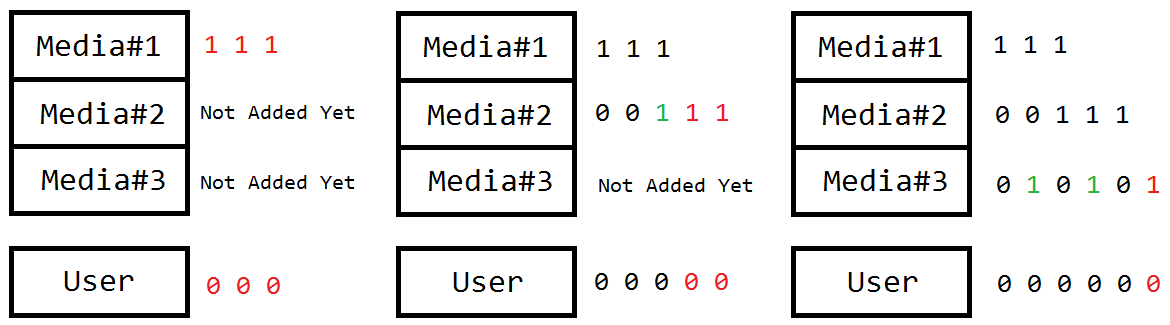
\includegraphics[width=0.8\textwidth]{Images/VectorUpdate.png}
\caption{Vector updates as new media is added}
\label{VectorUpdate}
\end{figure}

In the example above, each media is added to the collection one by one, with each addition all other media in the collection is updated as it is required. Red numbers indicate that the certain property was not yet part of the vectors, and therefore had to be added to all the media vectors. Green numbers indicate the certain property already was already in the vectors, and therefore did not have to update all the other media.

By comparing the vectors of a user with a media item, using the previously described cosine relation, there will be generated a coefficient, where the higher it is, the more similar is the two vectors. This is done by finding common points, and the respective length of both of the vectors, after which it is run through the cosine relation calculation.

\begin{table}[htb]
\centering
\begin{tabular}{|l||l|l|l|l|l|} \hline
	\textbf{Vector1} & 1 & 1 & 1 & 0 & 1 \\ \hline
	\textbf{Vector2} & 1 & 1 & 0 & 1 & 2 \\ \hline
\end{tabular}
\caption{Content Example}
\label{ContentEx}
\end{table}

See Table \ref{ContentEx} for an example. Finding the common points between the vectors is done by finding the dot product between them, which will give 4 in this case. Following that, the lengths will be found, which is the sum of each number squared, respectively resulting in 4 and 7. The common points is then divided by the lengths multiplied and square rooted, returning a coefficient for how similar the two vectors are. In this case it gives 0,756.

Following this, the media with the highest coefficients is chosen as recommendations generated by the content-based algorithm.